\input ../SlidePreamble
\input ../preamble

\newcommand{\solution}[1]{\bigskip {\bf Solution}: #1}

\begin{document}

{\Huge
  \centerline{\bf TTIC 31230, Fundamentals of Deep Learning}
  \bigskip
  \centerline{David McAllester, Winter 2018}
  \vfill
  \centerline{\bf Stochastic Gradient Descent (SGD)}
  \vfill
  \centerline{The Classical Convergence Thoerem}
  \vfill
  \centerline{RMSProp, Momentum and Adam}
  \vfill
  \centerline{Scaling Learning Rates with Batch Size}
  \vfill
  \centerline{Gradient Flow and Langevin Dynamics}
  
\slide{Vanilla SGD}

$$\Phi \;\minuseq\; \eta \hat{g}$$

\vfill
\begin{eqnarray*}
  \hat{g} & = & E_{(x,y) \sim \mathrm{Batch}}\;\nabla_\Phi\;\mathrm{loss}(\Phi,x,y) \\
  \\
  \\
  g & = & E_{(x,y) \sim \mathrm{Pop}}\;\nabla_\Phi\;\mathrm{loss}(\Phi,x,y) \\
\end{eqnarray*}

\slide{Issues}

\vfill
\begin{itemize}
\item {\bf Gradient Estimation.} The accuracy of $\hat{g}$ as an estimate of $g$.

  \vfill
\item {\bf Gradient Drift (second order structure).} The fact that $g$ changes as the parameters change.

  \vfill
\item {\bf Convergence.} To converge to a local optimum the learning rate must be gradually reduced toward zero.

  \vfill
  \item {\bf Exploration.} Since deep models are non-convex we need to search over the parameter space.  SGD can behave like MCMC.
\end{itemize}

\slide{A One Dimensional Example}

Suppose that $y$ is a scalar, and consider

\begin{eqnarray*}
 \mathrm{loss}(\beta,y) & = & \frac{1}{2}(\beta - y)^2 \\
 \\
  g & = &  \nabla_\beta\;E_{y \sim \mathrm{Pop}}\;\frac{1}{2}(\beta - y)^2 \\
  \\
  & = & \beta - E_{y \sim \mathrm{Pop}} \; y \\
  \\
  \hat{g} & = &\beta - E_{y \sim \mathrm{Batch}} \;y
\end{eqnarray*}

\vfill
Even if $\beta$ is optimal, for a finite batch we will have $\hat{g} \not = 0$.

\slide{The Classical Convergence Theorem}

$$\Phi \;\minuseq \; \eta_t \nabla_\Phi\;\mathrm{loss}(\Phi,x_t,y_t)$$

\vfill
For ``sufficiently smooth'' non-negative loss with

\vfill
$$\eta_t > 0\;\;\;\;\mbox{and}\;\;\;\;\lim_{t \rightarrow 0} \;\eta_t = 0\;\;\;\;\mbox{and}\;\;\;\;\sum_t \eta_t = \infty,$$

\vfill
we have that the training loss of $\Phi$ converges (in practice $\Phi$ converges to a local optimum of training loss).

\vfill
{\Large {\bf Rigor Police:} One can construct cases where $\Phi$ converges to a saddle point or even a limit cycle.}

\vfill
{\Large See ``Neuro-Dynamic Programming'' by Bertsekas and Tsitsiklis proposition 3.5.}

\slide{Physicist's Proof of the Convergence Theorem}

Since $\lim_{t \rightarrow 0} \;\eta_t = 0$ we will eventually get to arbitrarilly small learning rates.

\vfill
For sufficiently small learning rates any meaningful update of the parameters will be based on an arbitrarily large sample
of gradients at essentially the same parameter value.

\vfill
An arbitrarily large sample will become arbitrarily accurate as an estimate of the full gradient.

\vfill
But since $\sum_t \eta_t = \infty$, no matter how small the learning rate gets, we still can make arbitrarily large motions in parameter space.

\slidetwo{SGD as a form of MCMC}{Learning Rate as a Temperature Parameter}

\centerline{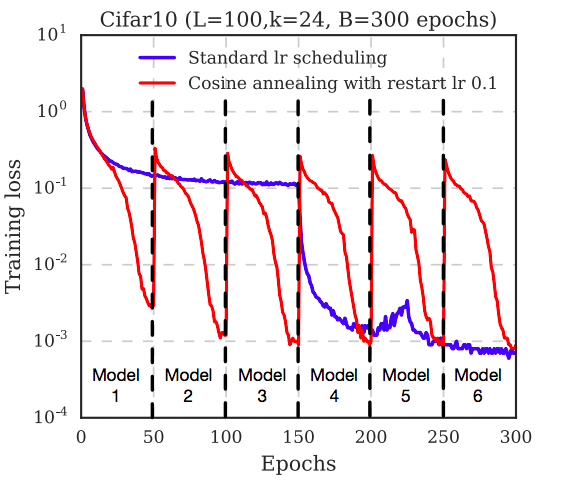
\includegraphics[height= 4in]{../images/AnnealingSGD}}
\centerline{\Large Gao Huang et. al., ICLR 2017}

\slide{}
\centerline{\bf Standard Non-Vanilla SGD Algorithms}
\vfill
\vfill

\slideplain{Digression on Running Averages}
Consider a sequence $x_1$, $x_2$, $x_3$, $\ldots$.
\vfill
For $t \geq N$, consider the average of the $N$ most recent values.
$$\tilde{\mu} = \frac{1}{N} \sum_{s=t-N+1}^t x_s$$

\vfill
This can be approximated more efficiently with
\begin{eqnarray*}
\hat{\mu}_0 & = & 0 \\
\\
\hat{\mu}_t & = & \left(1-\frac{1}{N}\right)\hat{\mu}_{t-1} + \left(\frac{1}{N}\right)x_t\;\;\;t \geq 1 \\
\\
\hat{\mu}_t & \approx & \tilde{\mu}_t \;\;\; t >N
\end{eqnarray*}

\slide{Running Averages}

More explicitly, for $\hat{\mu}_0 = 0$, the update

$$\hat{\mu}_t = \left(1-\frac{1}{N}\right)\hat{\mu}_{t-1} + \left(\frac{1}{N}\right)x_t$$

\vfill
gives

$$\hat{\mu}_t = \frac{1}{N} \sum_{1 \leq s \leq t} \left(1-\frac{1}{N}\right)^{-(t-s)} x_s$$

\vfill
where we have

$$\sum_{n\geq 0} \left(1-\frac{1}{N}\right)^{-n} = N$$

\slide{Momentum}

\begin{eqnarray*}
  {\color{red} v_t} & {\color{red} =} & {\color{red} \left(1-\frac{1}{N_g}\right) v_{t-1} + \eta * \hat{g}_t} \;\;\;\mbox{$N_g$ is typically 10 or 100}\\
  \\
  {\color{red} \Phi_{t+1}} & {\color{red} =} & {\color{red} \Phi_t -  v_t} \\
\end{eqnarray*}

The theory of momentum is generally given in terms of second order structure.


\centerline{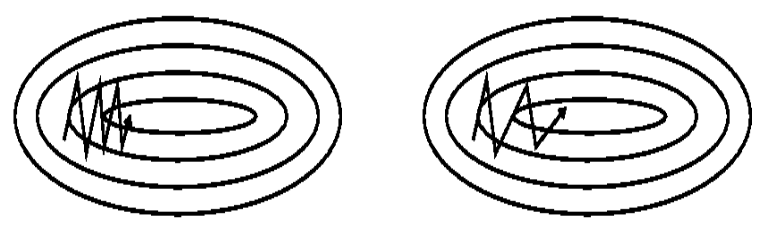
\includegraphics[width = 4in]{../images/momentum}}
\centerline{\Large Rudin's blog}

\slideplain{Momentum}

However, second order analyses are controversial in Deep Learning.

\vfill
We can perhaps get insight by reparameterizing the momentum equations.

\slide{We are Entering a Twilight Zone (TZ)}

\centerline{
\includegraphics[width = 6in]{../images/Twilight}}

\vfill
The twilight zone is material for which I do not know of a reference. 

\slide{Conjugacy of SGD Hyperparameters}

For an objective function $f(x,y)$ we say that $x$ and $y$ are conjugate if changing $x$ does effect the loss gradient for $y$.

\vfill
In other words if

{\color{red} $$\frac{\partial f(x,y)}{\partial x \partial y} = 0$$}

\vfill
We are seeking a nonlinear transformation on hyperparameters yielding robust conjugacy.

\slide{Solving for $\eta$ in terms of $N_g$ (TZ)}

Let $\eta'$ be a learning rate that is appropriate without momentum ($N_g = 1$).

\vfill
We will solve for a learning rate $\eta$ as a function of $N_g$ so as to minimize the perturbance of SGD
as we increase $N_g$.

\slide{An Equivalent Formulation of Momentum}

\begin{eqnarray*}
{\color{red} v_t} & = & \left(1-\frac{1}{N_g}\right) v_{t-1} + \eta \hat{g}_t \\
\\
& = & \left(1-\frac{1}{N_g}\right) v_{t-1} + \frac{1}{N_g}({\color{red} N_g\eta \hat{g}_t}) \\
\\
{\color{red} v_t} & = & {\color{red} N_g\eta\mu_t}\;\;\mbox{for}\;{\color{red} \mu_t = \left(1-\frac{1}{N_g}\right)\mu_{t-1} + \frac{1}{N_g} \hat{g}_t} \\
\\
\Phi_{t+1} & = & \Phi_t - v_t \\
\\
{\color{red} \Phi_{t+1}} & {\color{red} =} & {\color{red} \Phi_t - N_g\eta\mu_t} 
\end{eqnarray*}

\slide{Solving for $\eta$ (TZ)}

\begin{eqnarray*}
\mu_t & = &  \left(1-\frac{1}{N_g}\right)\mu_{t-1} + \frac{1}{N_g} \hat{g}_t \\
\\
\mbox{we have}\;\Phi_{t+1}& = & {\color{red} \Phi_t - N_g\eta\;\mu_t} \\
\\
\mbox{unperturbed is}\;\Phi_{t+1}& = & {\color{red} \Phi_t - \eta'\mu_t}
\end{eqnarray*}

\vfill
This gives {\color{red} $\eta = \eta'/N_g$}.

\vfill
We expect that that $\eta'$ and $N_g$ exhibit more independence (conjugacy) than $\eta$, $N_g$.

\slide{Scaling $\eta$ and $N_g$ with Batch Size}

Recent work has show that scaling hyper-parameters with the batch size can lead to effective learning with very large (highly parallel)
batches.

\vfill
{\bf Accurate, Large Minibatch SGD: Training ImageNet in 1 Hour}, Goyal et al., 2017.

\vfill
{\bf Don't Decay the Learning Rate, Increase the Batch Size}, Smith et al., 2018


\slide{Solving for $\eta$ as a Function of $B$}

Let $\eta'$ be a learning rate appropriate for $N_g = 1$ and $B = 1$.

\vfill
We will solve for $\eta$ as a function of $\eta'$ and $B$ so as to minimize the perturbance of SGD as we increase $B$.

\slide{Solving for $\eta$ as a function of $B$}

Consider two consecutive updates for a batch size of 1 with learning rate $\eta'$.

\begin{eqnarray*}
  \Phi_{t+1} & = & \Phi_t - \eta' \nabla_\Phi \mathrm{loss}(\Phi_t,x_t,y_t) \\
  \\
  \Phi_{t+2} & = & \Phi_{t+1} - \eta' \nabla_\Phi \mathrm{loss}({\color{red} \Phi_{t+1}},x_{t+1},y_{t+1}) \\\
  \\
  & \approx & \Phi_{t+1} - \eta' \nabla_\Phi \mathrm{loss}({\color{red} \Phi_t},x_{t+1},y_{t+1}) \\
  \\
  & = & \Phi_t - \eta'((\nabla_\Phi \mathrm{loss}(\Phi_t,x_t,y_t)) + (\nabla_\Phi \mathrm{loss}(\Phi_t,x_{t+1},y_{t+1})))
\end{eqnarray*}

\slide{Solving for $\eta$ as a function of $B$}

Let $\eta$ be the learning rate for batch size $B$.

\vfill
\begin{eqnarray*}
  \Phi_{t+2} & \approx & \Phi_t - \eta'((\nabla_\Phi \mathrm{loss}(\Phi_t,x_t,y_t)) + (\nabla_\Phi \mathrm{loss}(\Phi_t,x_{t+1},y_{t+1}))) \\
  \\
  & = & \Phi_t - 2\eta'\;\hat{g}\;\;\;\mathrm{for}\;\;B=2
\end{eqnarray*}

\vfill
We have {\color{red} $\Phi \;\minuseq \; \eta\;\hat{g}$}

\vfill
unperturbed is {\color{red} $\Phi \;\minuseq \; B\eta'\;\hat{g}$}

\vfill
This gives {\color{red} $\eta = B \eta'$}.

\vfill
We expect conjugacy for the parameters $\eta'$ and $B$.

\slide{Solving for $N_g$ as a Function of $B$}

Let $N'_g$ be a momentum parameter appropriate for $B=1$.

\vfill
We will solve for $N_g$ as a function of $B$ so as to minimize the perturbance of SGD as we increase $B$.

\vfill
For batch size $B$, $\hat{\mu}_t$ is an average of $\hat{g}$ over $N_gB$ gradient values.

\vfill
SGD seems minimally perturbed by
$$N_gB = N'_g\;\;\;\mbox{or}\;\;\;{\color{red} N_g = N'_g/B}$$

\vfill
We expect conjugacy for the parameters $N'_g$ and $B$.

\slide{Putting It Together (TZ)}

{\color{red}
\begin{eqnarray*}
N_g & = & \min(1,N'_g/B) \\
\\
\eta & = & B\eta'/N_g
\end{eqnarray*}
}

\vfill
We expect conjugacy for $\eta'$, $N'_g$ and $B$.

\slide{RMSProp}

RMSProp is based on a running average of $\hat{g}[i]^2$ for each real-valued model parameter $i$.

\begin{eqnarray*}
{\color{red} s_t[i]} & {\color{red} =} & {\color{red} \left(1-\frac{1}{N_s}\right) s_{t-1}[i] + \frac{1}{N_s} \hat{g}_t[i]^2}\;\;\;\mbox{$N_s$ typically 100 or 1000} \\
\\
{\color{red} \Phi_{t+1}[i]} & {\color{red} =} & {\color{red} \Phi_t[i] - \frac{\eta}{\sqrt{s_t[i] + \epsilon}}\;\; \hat{g}_t[i]}
\end{eqnarray*}


\slide{RMSProp}
\begin{eqnarray*}
{\color{red} s_t[i]} & {\color{red} =} & {\color{red} \left(1-\frac{1}{N_s}\right) s_{t-1}[i] + \frac{1}{N_s} \hat{g}_t[i]^2}\;\;\;\mbox{$N_s$ typically 100 or 1000} \\
\\
{\color{red} \Phi_{t+1}[i]} & {\color{red} =} & {\color{red} \Phi_t[i] - \frac{\eta}{\sqrt{s_t[i] + \epsilon}}\;\; \hat{g}_t[i]}
\end{eqnarray*}

\vfill
For $B = 1$ we have $s[i] \approx E\;\hat{g}[i]^2  =  g[i]^2 + \sigma[i]^2$

\vfill
We should expect $\sigma[i] >> g[i]$.

\vfill
We can therefore think of RMSProp as {\color{red} $\Phi[i] \;\minuseq\; \eta(\hat{g}[i]/\sigma[i])$}

\slide{RMSProp is Theoretically Mysterious}

{\color{red} $$\Phi[i] \;\minuseq \; \eta\;\frac{\hat{g}[i]}{\sigma[i]}\;\;(1)\hspace{5em}\Phi[i] \;\minuseq \; \eta\;\frac{\hat{g}[i]}{\sigma^2[i]}\;\;(2)$$}

\vfill
Although (1) seems to work better, (2) is better motivated theoretically.  To see this we can consider units.

\vfill
If parameters have units of ``weight'', and loss is in bits, then (2) type checks with $\eta$ having units of bits --- the numerical value of $\eta$
has no dependence on the choice of the weight unit.

\vfill
Consistent with the dimensional analysis, many theoretical analyses support (2) over (1) contrary to apparent empirical performance.

\slide{Scaling $\eta$ with Batch Size for RMSProp (TZ)}

Current RMSProp framework implementations do not scale well with batch size.

\vfill
The meaning of  $\hat{g}_i^2$ changes when increasing $B$.

\vfill
$\hat{g}_i$ is an average over a batch --- averaging reduces variance.

\begin{eqnarray*}
{\color{red} E\; \hat{g}_i^2} & {\color{red} =} & {\color{red} = \; \mu_i^2 + \frac{\sigma_i^2}{B}}
\end{eqnarray*}


\slide{Scaling $\eta$ with Batch Size for RMSProp (TZ)}

\begin{eqnarray*}
{\color{red} E\; \hat{g}_i^2} & {\color{red} = } &{\color{red} \mu_i^2 + \frac{\sigma_i^2}{B}}
\end{eqnarray*}

\vfill
To preserve the behavior of RMSProp while increasing $B$ we need a running average of $g_{b,i}^2$ for individual batch elements $b$.

\vfill
This requires augmenting backpropagation to compute an average (or sum) of $g_{b,i}^2$ as well as an average of
$g_{b,i}$ within each batch.

\slide{Adam --- Adaptive Momentum}

Adam combines momentum and RMSProp.

\vfill
It also uses ``bias correction'' of running averages.

\slide{A Digression on Bias Correction of Running Averages}

Consider a sequence $x_1,\;x_2,\;x_3,\ldots$ and consider the following for $N$ large.

\begin{eqnarray*}
\hat{\mu}_0 & = & 0 \\
\\
\hat{\mu}_t & = & \left(1-\frac{1}{N}\right)\hat{\mu}_{t-1} + \left(\frac{1}{N}\right)x_t
\end{eqnarray*}

\vfill
For $\mu \doteq E\;x$ we have $E\;\hat{\mu}_1 = \mu/N$.

\vfill
For $t << N$ we have $E\;\hat{\mu}_t \approx (t/N)\mu$.

\slide{Bias Correction of Running Averages}

The following running average maintains the invariant that $\hat{\mu}_t$ is exactly the average of $x_1,\ldots,x_t$.

\begin{eqnarray*}
\hat{\mu}_0 & = & 0 \\
\\
\hat{\mu}_t & = & \left(\frac{t-1}{t}\right)\hat{\mu}_{t-1} + \left(\frac{1}{t}\right)x_t \\
\\
\\
& = & \left(1-\frac{1}{t}\right)\hat{\mu}_{t-1} + \left(\frac{1}{t}\right)x_t
\end{eqnarray*}

\vfill
But this fails to track a moving average for $t >> N$.

\slide{Bias Correction of Running Averages}

The following avoids the initial bias toward zero while still tracking a moving average.

\begin{eqnarray*}
\hat{\mu}_0 & = & 0 \\
\\
\hat{\mu}_t & = & \left(1-\frac{1}{\min(N,t)}\right)\hat{\mu}_{t-1} + \left(\frac{1}{\min(N,t)}\right)x_t
\end{eqnarray*}

\vfill
The published version of Adam has a more obscure form of bias correction which yields essentially the same effect.

\slide{Adam (simplified)}

\begin{eqnarray*}
  \mu_0[i] & = & s_0[i] = 0 \\
  \\
  \mu_{t}[i] & = & \left(1-\frac{1}{\min(t,N_g)}\right)\mu_{t-1}[i] + \frac{1}{\min(t,N_g)} \hat{g}_t[i] \\
  \\
  s_{t}[i] & = & \left(1-\frac{1}{\min(t,N_s)}\right)s_{t-1}[i] + \frac{1}{\min(t,N_s)} \hat{g}_t[i]^2 \\
  \\
\Phi_{t+1}[i] & =  & \Phi_t - \frac{\eta}{\sqrt{s_{t}[i] + \epsilon}}\;\;\mu_{t}[i]
\end{eqnarray*}

\slide{Annealing the Learning Rate}

\centerline{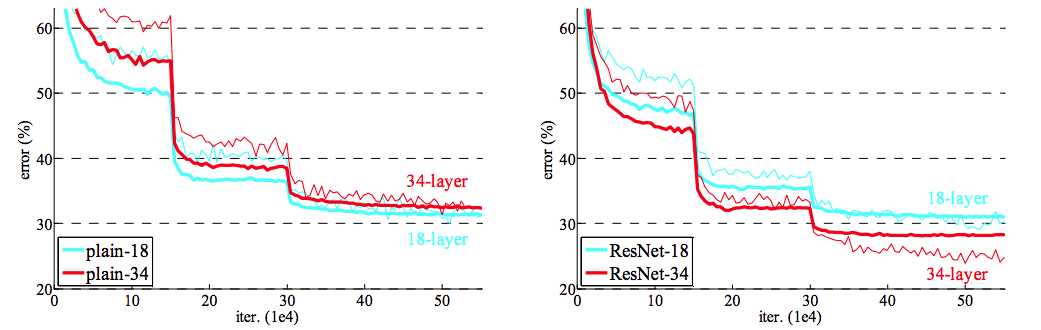
\includegraphics[width = 7in]{../images/annealing}}

\vfill
These Plots are from the original ResNet paper.  Left plot is for CNNs without residual skip connections, the right plot is ResNet.

\vfill
Thin lines are training error, thick lines are validataion error.

\vfill
In all cases $\eta$ is reduced twice, each time by a factor of 2.

\slide{A Quadratic Basin Annealing Theorem (TZ)}

\vfill
In practice annealed SGD will converge to a local optimum.

\vfill
We consider stationary distributions restricted to a neighborhood of a (local) optimim $\Phi^*$ satisfying

\begin{eqnarray*}
{\cal L}(\Phi) & = & E_i\;{\cal L}_i(\Phi) \\
\\
{\cal L}_i(\Phi^* + \Delta \Phi) & = & {\cal L}_i + g_i \Delta \Phi + \frac{1}{2} \Delta\Phi^\top H_i \Delta\Phi \\
\\
E_i\; g_i & = & 0\\
\\
E_i\; H_i & & \mbox{is positive definite}
\end{eqnarray*}

\slide{A Quadratic Basin Annealing Theorem (TZ)}

Theorem:

$${\cal L}(0) = {\cal L}(\Phi^*)\;\;\;\;\;\;\;\;\;\;\;\;{\color{red} \left.\frac{\partial {\cal L}(\eta)}{\partial \eta}\right|_{\eta = 0} \;\;=\;\; \frac{1}{4}\; E_i\; ||g_i||^2}$$

\slide{Analyzing Stationary Distributions (TZ)}

$${\cal L}(\eta) \approx {\cal L}(\Phi^*) + \eta \left(E_I ||g_i||^2\right)$$

\vfill
$${\cal L}(\Phi^*) = {\cal L}(\eta) - 2({\cal L}(\eta) - {\cal L}(\eta/2)) = 2{\cal L}(\eta/2) - {\cal L}(\eta)$$

\vfill
\centerline{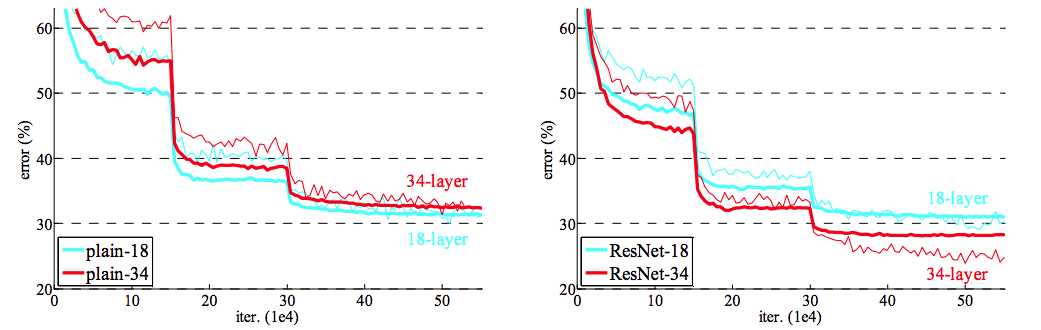
\includegraphics[width = 7in]{../images/annealing}}

\slide{Proof: Observation 1 (TZ)}

\begin{eqnarray*}
{\cal L}(\eta) & = & \;\;\; E_{\Delta \Phi \sim P_\eta}\;E_i \;\;\;\; {\cal L}_i + g_i\Delta _\Phi + \frac{1}{2}\;\Delta \Phi^\top H_i \Delta \Phi \\
\\
& = & E_i\; {\cal L}_i + E_{\Delta \Phi \sim P_\eta} \;\;\;\;(E_i\;g_i) \;\Delta \Phi + \frac{1}{2}\;\Delta \Phi^\top (E_i\; H_i) \Delta \Phi \\
\\
& = & {\cal L}(\Phi^*)\;\; + \;\; E_{\Delta \Phi \sim P_\eta}\;\;\;\frac{1}{2}\;\Delta \Phi^\top (E_i\;H_i) \Delta \Phi
\end{eqnarray*}

\slide{Proof: Step 1 (TZ)}
Because $P_\eta$ is a stationary distribution we must have

$$E_{\Delta \Phi \sim P_\eta}E_i\; ||\Delta \Phi - \eta (g_i + H_i\Delta \Phi)||^2 = E_{\Delta \Phi \sim P_\eta}\; ||\Delta \Phi||^2$$

\vfill
$$E_{\Delta \Phi \sim P_\eta}E_i\;-2\eta \Delta \Phi^\top (g_i + H_i\Delta \Phi) +\eta^2||(g_i + H_i\Delta \Phi)||^2 = 0$$

\vfill
$$E_{\Delta \Phi \sim P_\eta}\;\left(\frac{1}{2}\Delta \Phi^\top (E_i \;H_i)\Delta \Phi\right) = \frac{\eta}{4}\;E_{\Delta \Phi \sim P_\eta}E_i \;||(g_i + H_i\Delta \Phi)||^2$$

\vfill
$${\color{red} {\cal L}(\eta)  = {\cal L}(\Phi^*) + \frac{\eta}{4}\;E_{\Delta \Phi \sim P_\eta}E_i \;||(g_i + H_i\Delta \Phi)||^2}$$

\slide{Proof Step 2 (TZ)}

\begin{eqnarray*}
{\color{red} {\cal L}(\eta)}  & {\color{red} =} & {\color{red} {\cal L}(\Phi^*) + \frac{\eta}{4}\;E_{\Delta \Phi \sim P_\eta}E_i \;||(g_i + H_i\Delta \Phi)||^2} \\
\\
{\color{red} \left.\frac{\partial {\cal L}(\eta)}{\partial \eta}\right|_{\eta = 0}} & = & \frac{1}{4} \; \lim_{\eta \rightarrow 0} \; E_{\Delta \Phi \sim P_\eta}\; E_i \;||(g_i + H_i\Delta \Phi)||^2 \\
\\
\\
& = & \frac{1}{4} \; E_i\;\lim_{\eta \rightarrow 0}\;E_{\Delta \Phi \sim P_\eta} \;||(g_i + H_i\Delta \Phi)||^2 \\
\\
\\
& {\color{red} =} & {\color{red} \frac{1}{4}\; E_i\;||g_i||^2}
\end{eqnarray*}

\slide{Gradient Flow}

Consider the differential equation

$${\color{red} \frac{d \Phi}{d t} = - g(\Phi) \;\;\;\;\;\; g(\Phi) = \nabla_\Phi\; E_{(x,y) \sim \mathrm{Train}}\;{\cal L}(\Phi,x,y)}$$

\vfill
Let $\Phi(t)$ be the solution satisfying $\Phi(0) = \Phi_{\mathrm{init}}$.

\vfill
For small values of $\Delta t$ this differential equation can be approximated by

\vfill
$${\color{red} \Delta \Phi = - g(\Phi)\Delta t}$$

\vfill
Here $\Delta t$ can be interpreted as a learning rate.

\slide{Gradient Flow}

$${\color{red} \Delta \Phi = - g(\Phi)\Delta t}$$

\vfill
For a given value of $t$ and $N$ let $\Phi_j$ be defined by

\vfill
\begin{eqnarray*}
\Phi_0 & = & \Phi_{\mathrm{init}} \\
\\
\Phi_{j+1} & = & \Phi_j - \left(\frac{t}{N}\right) g(\Phi_j)
\end{eqnarray*}

\vfill
$${\color{red} \lim_{N\rightarrow \infty} \;\Phi_N = \Phi(t)}$$


\slide{Progress Theorem for Gradient Flow}

\begin{eqnarray*}
  \frac{d \ell}{d t} & = & (\nabla_\Phi \;\ell(\Phi)) \cdot \frac{d \Phi}{dt} \\
  \\
  & = & - (\nabla_\Phi \;\ell(\Phi)) \cdot (\nabla_\Phi \;\ell(\Phi)) \\
  \\
  & = & - ||\nabla_\Phi \;\ell(\Phi)||^2 \\
  \\
  & \leq & 0
\end{eqnarray*}

\vfill
If $\ell(\Phi) \geq 0$ then $\ell(\Phi)$ must converge to a limiting value.

\vfill
This does not imply that $\Phi$ converges.

\slide{SGD also yields Gradient Flow}
For
$$\Phi_{j+1} = \Phi_j - \left(\frac{t}{N}\right) {\color{red} \hat{g}_j}$$
we still have

\vfill
$${\color{red} \lim_{N\rightarrow \infty} \;\Phi_N = \Phi(t)}$$

\vfill
To see this note that we can divide the updates into $\sqrt{N}$ blocks each of size $\sqrt{N}$.  The ``time'' spent within each block is $t/\sqrt{N}$ which converges to 0.
But the number of updates within each block grows as $\sqrt{N}$ and hence the average update within a block converges to $g$.


\slide{Langevin Dynamics}

Consider SGD with $B = 1$.

$$\Phi \;\minuseq\; \eta\hat{g}$$

\vfill
As with gradient flow, for $N$ steps of SGD we define $t = N \eta$.

\vfill
In Langevin dynamics we hold $\eta > 0$ fixed.

\vfill
We then consider $\Delta t$ large compared to $\eta$ (so that it corresponds to many SGD updates) but
small enough so that the gradient distribution does not change during the interval $\Delta t$.

\slide{Langevin Dynamics}

If the mean gradient $g(\Phi)$ is approximately constant over the interval $\Delta t = N \eta$ we have

$$\Phi(t + \Delta t)  \approx \Phi(t) -g(\Phi)\Delta t + \eta \sum_{j=1}^N (g(\Phi) - \hat{g}_i)$$

\vfill
The Random variables in the last term have zero mean.

\vfill
By the law of large numbers a sum (not the average) of $N$ random vectors will approximate a Gaussian distribution where the standard deviation
grows like $\sqrt{N}$.

\slide{Langevin Dynamics}

Let $\Sigma$ be the covariance matrix of the random variable $\hat{g}$ and assume this is approximately constant over the interval $\Delta t$.

\vfill
Let $\epsilon$ be a zero mean Gaussian random variable with the same covariance matrix $\Sigma$.

\begin{eqnarray*}
\Phi(t + \Delta t) & \approx & \Phi(t) -g(\Phi)\Delta t + \eta \sum_{j=1}^N (g(\Phi) - \hat{g}_i) \\
\\
& \approx & \Phi(t) -g(\Phi)\Delta t + \eta \epsilon \sqrt{N} \\
\\
& = & \Phi(t) -g(\Phi)\Delta t + \eta \epsilon \sqrt{\frac{\Delta t}{\eta}}
\end{eqnarray*}


\slide{Langevin Dynamics}

\begin{eqnarray*}
\Phi(t + \Delta t) & \approx & \Phi(t) -g(\Phi)\Delta t + \sqrt{\eta} \epsilon \sqrt{\Delta t}\;\;\;\;\;\; \epsilon \sim {\cal N}(0,\Sigma)
\end{eqnarray*}

\vfill
This can be modeled by a continuous time stochastic process --- Langevin dynamics --- defined by the notation

$$d\Phi =  -g(\Phi)dt + \sqrt{\eta} \epsilon \sqrt{dt}\;\;\;\;\;\; \epsilon \sim {\cal N}(0,\Sigma)$$

\vfill
This is a stochastic differential equation.

\vfill
If ${\cal L}$ is constant and $\Sigma = I$ we get Brownian motion.

\slide{Langevin Dynamics}

\begin{eqnarray*}
\Phi(t + \Delta t) & \approx & \Phi(t) -g(\Phi)\Delta t + \sqrt{\Delta t\; \eta}\;\epsilon\;\;\;\;\;\; \epsilon \sim {\cal N}(0,\Sigma)
\end{eqnarray*}

\vfill
Note that for $\eta \rightarrow 0$ the noise term vanishes.  If we then take $\Delta t \rightarrow 0$ (at a slower rate) we are back to gradient flow.

\vfill
In Langevin dynamics we hold $\eta > 0 $ fixed.

\slide{Stationary Distributions}

SGD at $B = 1$ defines a Markov process

$$\Phi \;\minuseq \; \eta \hat{g}$$

\vfill
Under Langevin dynamics the stationary distribution is a continuous density in parameter space.

\vfill
If the covariance matrix is isotropic (all eigenvalues are the same) we get a Gibbs distribution.


\slide{The 1-D Langevin Stationary Distribution}

Consider SGD on a single parameter.

\vfill
Let $p$ be a probability density on $x$.

\vfill
Assume that the gradient $\hat{g}$ has variance $\sigma$ everywhere.

\vfill
There is a diffusion flow proportional to $\eta^2\sigma^2\;dp/dx$.

\vfill
There is a gradient flow equal to $\eta p \;d {\cal L}/dx$.

\vfill
For a stationary distribution the two flows cancel giving.

\vfill
{\color{red} $$\alpha \eta^2 \sigma^2 \frac{dp}{dx} = - \eta p\frac{d{\cal L}}{dx}$$}


\slide{The 1-D Langevin Stationary Distribution}

\vspace{-2ex}
\begin{eqnarray*}
\alpha \eta^2 \sigma^2 \frac{dp}{dx} & = & - \eta p\frac{d{\cal L}}{dx} \\
\\
\frac{dp}{p} & = & \frac{-d{\cal L}}{\alpha\eta\sigma^2} \\
\\
\ln p & = & \frac{-{\cal L}}{\alpha \eta \sigma^2} + C \\
\\
{\color{red} p(x)} & = & {\color{red} \frac{1}{Z}\exp\left(\frac{-{\cal L}(x)}{\alpha \eta \sigma^2}\right)}\;\;\alpha \approx 1/10
\end{eqnarray*}

\vfill
We get a Gibbs distribution!

\slide{A 2-D Langevin Stationary Distribution}

Let $p$ be a probability density on two parameters $(x,y)$.

\vfill
We consider the case where $x$ and $y$ are completely independent with
$${\cal L}(x,y) = {\cal L}(x) + {\cal L}(y)$$

\vfill
For completely independent variables we have
\begin{eqnarray*}
p(x,y) & = & p(x)p(y) \\
\\
&= & \frac{1}{Z} \exp\left(\frac{-{\cal L}(x)}{\alpha \eta \sigma_x^2} + \frac{-{\cal L}(y)}{\alpha \eta \sigma_y^2}\right)
\end{eqnarray*}

\slide{A 2-D Langevin Stationary Distribution}

\begin{eqnarray*}
p(x,y) & = & \frac{1}{Z} \exp\left(\frac{-{\cal L}(x)}{\alpha \eta \sigma_x^2} + \frac{-{\cal L}(y)}{\alpha \eta \sigma_y^2}\right) \\
\\
\\
& = & \frac{1}{Z} \exp\left(-\beta_x{\cal L}(x) - \beta_y{\cal L}(y)\right)
\end{eqnarray*}

\vfill
This is not a Gibbs distribution!

\vfill
It has two different temperature parameters!

\slide{Langevin and RMSProp}

Suppose we use parameter-specific learning rates $\eta_x$ and $\eta_y$

\begin{eqnarray*}
p(x,y) & = & \frac{1}{Z} \exp\left(\frac{-{\cal L}(x)}{\alpha \eta_x \sigma_x^2} + \frac{-{\cal L}(y)}{\alpha \eta_y \sigma_y^2}\right)
\end{eqnarray*}

Setting $\eta_x = \eta'/\sigma^2_x$ and $\eta_y = \eta'/\sigma^2_y$ gives

\begin{eqnarray*}
p(x,y) & = & \frac{1}{Z} \exp\left(\frac{-{\cal L}(x)}{\alpha \eta'} + \frac{-{\cal L}(y)}{\alpha \eta'}\right) \\
\\
& = & \frac{1}{Z} \exp\left(\frac{-{\cal L}(x,y)}{\alpha \eta'}\right)\;\;\;\mathrm{Gibbs!}
\end{eqnarray*}

\vfill
RMSProp sets $\eta_x = \eta'/\sigma_x$ rather than $\eta_x = \eta'/\sigma_x^2$.  Empirically this seems better.

\slideplain{Annealing Langevin Stationary Distributions}

Although the stationary distribution is not a Boltzman distribution, the learning rate $\eta$ acts as a temperature parameter giving an eiganvalue-dependent temperature for each eigenvector
of the noise covariance $\Sigma$.

\vfill
Let $P_\eta$ be the stationary distribution at learning rate $\eta$.

\begin{eqnarray*}
{\cal L}(\Phi) & = & E_i\;{\cal L}_i(\Phi) \\
\\
{\cal L}(\eta) & = & E_{\Phi \sim P_\eta}\;{\cal L}(\Phi) \\
\\
\lim_{\eta \rightarrow 0} {\cal L}(\eta) & = & {\cal L}(\Phi^*)\;\;\;\mbox{for Langevin dynamics}
\end{eqnarray*}


\ignore{
\slide{An Original Algorithm Derivation}

\vfill
We will derive a learning rate by maximizing a lower bound on the rate of reduction in training loss.

\vfill
We must consider

\vfill
\begin{itemize}
\item {\bf Gradient Estimation.} The accuracy of $\hat{g}$ as an estimate of $g$.

  \vfill
\item {\bf Gradient Drift (second order structure).} The fact that $g$ changes as the parameters change.
\end{itemize}

\slide{Analysis Plan}

We will calculate a batch size $B^*$ and learning rate $\eta^*$ by optimizing an improvement guarantee for a single batch update.

\vfill
We then use learning rate scaling to derive the learning rate  $\eta_B$ for a batch size $B << B^*$.

\slide{Deriving Learning Rates}

If we can calculate $B^*$ and $\eta^*$ for optimal loss reduction in a single batch
we can calculate $\eta_B$.

\vfill
$$\eta_B = B\;\eta_1$$

\vfill
$$\eta^* = B^* \eta_1$$

\vfill
$$\eta_1 = \frac{\eta^*}{B^*}$$

\vfill
$${\color{red} \eta_B = \frac{B}{B^*} \;\eta^*}$$

\slide{Calculating $B^*$ and $\eta^*$ in One Dimension}

We will first calculate values $B^*$ and $\eta^*$ by optimizing the loss reduction over a single batch update in one dimension.

\vfill
\begin{eqnarray*}
  g & = & \hat{g} \pm \frac{2\hat{\sigma}}{\sqrt{B}} \\
  \\
  \\
  \\
  \hat{\sigma} & = & \sqrt{E_{(x,y) \sim \mathrm{Batch}} \left(\frac{d\;\mathrm{loss}(\beta,x,y)}{d \beta} - \hat{g}\right)^2}
\end{eqnarray*}

\slide{The Second Derivative of $\mathrm{loss}(\beta)$}

\begin{eqnarray*}
  \mathrm{loss}(\beta) & = & E_{(x,y) \sim \mathrm{Train}}\;\mathrm{loss}(\beta,x,y) \\
  \\
  d^2 \mathrm{loss}(\beta)/d \beta^2 & \leq & L \;\;\;\mbox{\Large (Assumption)} \\
  \\
  \mathrm{loss}(\beta - \Delta\beta) & \leq & \mathrm{loss}(\beta) - g\Delta \beta + \frac{1}{2}L\Delta \beta^2 \\
  \\
  \\
  \mathrm{loss}(\beta - \eta\hat{g}) & \leq & \mathrm{loss}(\beta) - g(\eta\hat{g}) + \frac{1}{2}L(\eta\hat{g})^2
\end{eqnarray*}

\slide{A Progress Guarantee}

\begin{eqnarray*}
  \mathrm{loss}(\beta - \eta\hat{g}) & \leq & \mathrm{loss}(\beta) - g(\eta\hat{g}) + \frac{1}{2}L(\eta\hat{g})^2 \\
  \\
  \\
  & = &  \mathrm{loss}(\beta) - \eta (\hat{g} - (\hat{g} -g)) \hat{g} + \frac{1}{2}L\eta^2 \hat{g}^2 \\
  \\
  \\
  & \leq &  \mathrm{loss}(\beta) - \eta \left(\hat{g} - \frac{2\hat{\sigma}}{\sqrt{B}}\right)\hat{g} + \frac{1}{2}L \eta^2 \hat{g}^2
\end{eqnarray*}

\slideplain{Optimizing $B$ and $\eta$}

$$\mathrm{loss}(\beta - \eta\hat{g}) \leq \mathrm{loss}(\beta) - \eta \left(\hat{g} - \frac{2\hat{\sigma}}{\sqrt{B}} \right)\hat{g}  + \frac{1}{2}L \eta^2 \hat{g}^2$$

\vfill
We optimize progress per gradient calculation by optimizing the right hand side divided by $B$.  The derivation at the end of the slides gives

\vfill
$$B^*  =  \frac{16\hat{\sigma}^2}{\hat{g}^2},\;\;\;\;\eta^*  =  \frac{1}{2L}$$

\vfill
$${\color{red} \eta_B} = \frac{B}{B^*} \eta^* = {\color{red} \frac{B \hat{g}^2}{32\hat{\sigma}^2L}}$$

\vfill
Recall this is all just in one dimension.

\slide{Estimating $\hat{g}_{B^*}$ and $\hat{\sigma}_{B^*}$}

$${\color{red} \eta_B = \frac{B \hat{g}^2}{32\hat{\sigma}^2L}}$$

\vfill
We are left with the problem that $\hat{g}$ and $\hat{\sigma}$ are defined in terms of batch size $B^* >> B$.

\vfill
We can estimate $\hat{g}_{B^*}$ and $\hat{\sigma}_{B^*}$ using a running average with a time constant corresponding to $B^*$.

\slide{Estimating $\hat{g}_{B^*}$}

\begin{eqnarray*}
  \hat{g}_{B^*} & = & \frac{1}{B^*} \sum_{(x,y) \sim \mathrm{Batch}(B^*)}\; \frac{d\;\mathrm{Loss}(\beta,x,y)}{d\beta} \\
  \\
  \\
  & = & \frac{1}{N} \sum_{s=t-N+1}^t \hat{g}^s\;\;\;\;\;\mbox{with}\;N= \frac{B^*}{B} \;\mbox{for batch size}\;B \\
  \\
  \\
  \tilde{g}^{t+1} & = & \left(1-\frac{B}{B^*}\right)\tilde{g}^t + \frac{B}{B^*} \hat{g}^{t+1}
\end{eqnarray*}

\vfill
We are still working in just one dimension.

\slide{A Complete Calculation of $\eta$ (in One Dimension)}
\begin{eqnarray*}
  \tilde{g}^{t+1} & = & \left(1-\frac{B}{B^*(t)}\right)\tilde{g}^t + \frac{B}{B^*(t)} \hat{g}^{t+1} \\
  \\
  \tilde{s}^{t+1} & = & \left(1-\frac{B}{B^*(t)}\right)\tilde{s}^t + \frac{B}{B^*(t)} (\hat{g}^{t+1})^2 \\
  \\
  \tilde{\sigma}^t & = & \sqrt{\tilde{s}^t - (\tilde{g}^t)^2} \\
  \\
  B^*(t) &= & \left\{\begin{array}{ll} K & \mbox{for}\;\; t \leq K \\
  16(\tilde{\sigma}^t)^2/((\tilde{g}^t)^2 + \epsilon) & \mbox{otherwise} \end{array}\right.
\end{eqnarray*}

\slide{A Complete Calculation of $\eta$ (in One Dimension)}

$$\eta^t = \left\{\begin{array}{ll} 0 & \mbox{for}\;\;t \leq K \\ \frac{(\tilde{g}^t)^2}{32(\tilde{\sigma}^t)^2L} & \mbox{otherwise}
\end{array}\right.$$

\vfill
As $t \rightarrow \infty$ we expect $\tilde{g}^t \rightarrow 0$ and $\tilde{\sigma}^t \rightarrow \sigma > 0$ which implies
$\eta^t \rightarrow 0$.

\slide{The High Dimensional Case}

So far we have been considering just one dimension.

\vfill
We now propose treating each dimension $\Phi[i]$ of a high dimensional parameter vector $\Phi$ independently using the one dimensional analysis.

\vfill
We can calculate $B^*[i]$ and $\eta^*[i]$ {\bf for each individual parameter} $\Phi[i]$.

\vfill
Of course the actual batch size $B$ will be the same for all parameters.

\slide{A Complete Algorithm}
\begin{eqnarray*}
  \tilde{g}^{t+1}[i] & = & \left(1-\frac{B}{B^*(t)[i]}\right)\tilde{g}^t[i] + \frac{B}{B^*(t)[i]} \hat{g}^{t+1}[i] \\
  \\
  \tilde{s}^{t+1}[i] & = & \left(1-\frac{B}{B^*(t)[i]}\right)\tilde{s}^t[i] + \frac{B}{B^*(t)[i]} \hat{g}^{t+1}[i]^2 \\
  \\
  \tilde{\sigma}^t[i] & = & \sqrt{\tilde{s}^t[i] - \tilde{g}^t[i]^2} \\
  \\
  B^*(t)[i] &= & \left\{\begin{array}{ll} K & \mbox{for}\;\; t \leq K \\
  \lambda_B\tilde{\sigma}^t[i]^2/(\tilde{g}^t[i]^2 + \epsilon) & \mbox{otherwise} \end{array}\right.
\end{eqnarray*}

\slide{A Complete Algorithm}

$$\eta^t[i] = \left\{\begin{array}{ll} 0 & \mbox{for}\;\;t \leq K \\
        \frac{\lambda_\eta\tilde{g}^t[i]^2}{\tilde{\sigma}^t[i]^2} & \mbox{otherwise}
\end{array}\right.$$

\vfill
$$\Phi^{t+1}[i] = \Phi^t[i] - \eta^t[i] \hat{g}^t[i]$$

\vfill
Here we have meta-parameters $K$, $\lambda_B$, $\epsilon$ and $\lambda_\eta$.

\slideplain{Appendix: Optimizing $B$ and $\eta$}

$$\mathrm{loss}(\beta - \eta\hat{g}) \leq \mathrm{loss}(\beta) - \eta \hat{g}\left(\hat{g} - \frac{2\hat{\sigma}}{\sqrt{B}} \right)  + \frac{1}{2}L \eta^2 \hat{g}^2$$

Optimizing $\eta$ we get

\begin{eqnarray*}
 \hat{g}\left(\hat{g} - \frac{2\hat{\sigma}}{\sqrt{B}} \right) & = & L \eta \hat{g}^2
\end{eqnarray*}


\begin{eqnarray*}
\eta^*(B) & = & \frac{1}{L}\left(1 - \frac{2\hat{\sigma}}{\hat{g}\sqrt{B}}\right)
\end{eqnarray*}

\vfill
Inserting this into the guarantee gives
$$\mathrm{loss}(\Phi - \eta \hat{g}) \leq \mathrm{loss}(\Phi) - \frac{L}{2}\eta^*(B)^2\hat{g}^2$$

\slide{Optimizing $B$}

Optimizing progress per sample, or maximizing $\eta^*(B)^2/B$, we get

\begin{eqnarray*}
\frac{\eta^*(B)^2}{B} & = & \frac{1}{L^2}\left(\frac{1}{\sqrt{B}} - \frac{2\hat{\sigma}}{\hat{g}B}\right)^2 \\
\\
0 & = &  - \frac{1}{2} B^{-\frac{3}{2}} + \frac{2\hat{\sigma}}{\hat{g}} B^{-2} \nonumber \\
\\
B^* & = & \frac{16\hat{\sigma}^2}{\hat{g}^2} \\
\\
\eta^*(B^*) = \eta^*  & = & \frac{1}{2L}
\end{eqnarray*}

\slide{Appendix II: A Formal Bound for the Vector Case}

We will prove that minibatch SGD for a {\bf sufficiently large batch size} (for gradient estimation) and a {\bf sufficient small learning rate} (to avoid gradient drift)
is guaranteed (with high probability) to reduce the loss.

\vfill
This guarantee has two main requirements.

\vfill
\begin{itemize}
\item A smoothness condition to limit gradient drift.

  \vfill
\item A bound on the gradient norm allowing high confidence gradient estimation.
\end{itemize}
  

\slide{Smoothness: The Hessian}

We can make a second order approximation to the loss.

\begin{eqnarray*}
  \ell(\Phi + \Delta \Phi) & \approx & \ell(\Phi) + g^\top \Delta \Phi + \frac{1}{2} \Delta \Phi^\top H \Delta \Phi \\
  \\
  g & = & \nabla_\Phi\;\ell(\Phi) \\
  \\
  H & = & \nabla_\Phi \nabla_\Phi\; \ell(\Phi)
\end{eqnarray*}


\slide{The Smoothness Condition}

We will assume

$$||H\Delta \Phi|| \leq L||\Delta \Phi||$$

We now have

\vfill
$$\Delta \Phi^\top H \Delta \Phi \leq L ||\Delta \Phi||^2$$

\vfill
Using the second order mean value theorem one can prove

\begin{eqnarray*}
  \ell(\Phi + \Delta \Phi)  & \leq &    \ell(\Phi) + g^\top \Delta \Phi + \frac{1}{2} L ||\Delta \Phi||^2
\end{eqnarray*}


\slide{A Concentration Inequality for Gradient Estimation}

Consider a vector mean estimator where the vectors $g_n$ are drawn IID.

$$g_n = \nabla_\Phi \ell_n(\Phi) \;\;\;\;\;\;\hat{g} = \frac{1}{k} \sum_{n=1}^k g_n \;\;\;\; \;\;\;\;\;\;\;\; g = \expectsub{n}{\nabla_\Phi\;\ell_n(\Phi)}$$

\vfill
{\bf If with probability 1 over the draw of $n$ we have $|(g_n)_i - g_i| \leq b$ for all $i$} then with probability of at least $1-\delta$ over the draw of the sample

\vfill

$$||\hat{g} - g|| \leq \frac{\eta}{\sqrt{k}} \;\;\;\;\;\;\;\;\;\;\;\;\;\; \eta = b\left(1 + \sqrt{2 \ln (1/ \delta) }\right)$$


\vfill
{\huge Norkin and Wets ``Law of Small Numbers as Concentration Inequalities ...'', 2012, theorem 3.1}

\begin{eqnarray*}
 \ell(\Phi + \Delta \Phi) & \leq &   \ell(\Phi) + g^\top \Delta \Phi + \frac{1}{2} L ||\Delta \Phi||^2 \\
  \\
\ell(\Phi - \eta\widehat{g}) & \leq & \ell(\Phi) - \eta g^\top \widehat{g} + \frac{1}{2}L \eta^2 ||\widehat{g}||^2\\
  \\
  & = &  \ell(\Phi) - \eta (\widehat{g} - (\widehat{g} -g))^\top \widehat{g} + \frac{1}{2}L\eta^2 ||\widehat{g}||^2 \\
  \\
  & = &  \ell(\Phi) - \eta ||\widehat{g}||^2 + \eta(\widehat{g} -g)^\top \widehat{g} + \frac{1}{2}L \eta^2 ||\widehat{g}||^2 \\
  \\
  & \leq &  \ell(\Phi) - \eta ||\widehat{g}||^2 + \eta\frac{\eta}{\sqrt{k}}||\widehat{g}|| + \frac{1}{2}L \eta^2 ||\widehat{g}||^2 \\
  \\
  & = & \ell(\Phi) - \eta ||\widehat{g}||\left(||\widehat{g}|| - \frac{\eta}{\sqrt{k}} \right)  + \frac{1}{2}L \eta^2 ||\widehat{g}||^2 \\
\end{eqnarray*}

\slideplain{Optimizing $\eta$}

Optimizing $\eta$ we get

\begin{eqnarray*}
 ||\widehat{g}||\left(||\widehat{g}|| - \frac{\eta}{\sqrt{k}} \right) & = & - L \eta ||\widehat{g}||^2
\end{eqnarray*}


\begin{eqnarray*}
\eta & = & \frac{1}{L}\left(1 - \frac{\eta}{||\widehat{g}||\sqrt{k}}\right)
\end{eqnarray*}

\vfill
Inserting this into the guarantee gives
$$\ell(\Phi - \eta \widehat{g}) \leq \ell(\Phi) - \frac{L}{2}\eta^2||\widehat{g}||^2$$

\slide{Optimizing $k$}

Optimizing progress per sample, or maximizing $\eta^2/k$, we get.

\begin{eqnarray*}
\frac{\eta^2}{k} & = & \frac{1}{L^2}\left(\frac{1}{\sqrt{k}} - \frac{2\hat{\sigma}}{||\widehat{g}||k}\right)^2 \\
\\
0 & = &  - \frac{1}{2} k^{-\frac{3}{2}} + \frac{2\hat{\sigma}}{||\widehat{g}||} k^{-2} \nonumber \\
\\
k & = & \left(\frac{22\hat{\sigma}}{||\widehat{g}||}\right)^2 \\
\\
\eta & = & \frac{1}{2L}
\end{eqnarray*}
}


\slide{END}

} \end{document}

